\documentclass{article}

\usepackage[utf8]{inputenc}
\usepackage[T1]{fontenc}
\usepackage{lipsum}
\usepackage{graphicx}
\usepackage{amsmath}
\usepackage[margin=1in]{geometry}
\usepackage{titlesec}
\usepackage{enumitem}

\titleformat{\section} 
{\LARGE\bfseries}{\thesection}{1em}{}

\titleformat{\subsection} 
{\Large\bfseries}{\thesection}{1em}{}

\begin{document}

\pagestyle{empty}

\section*{Normalizzazione} 
\large

Le \textbf{ridondanze} sui dati possono essere di due tipi:
\begin{itemize}[label={-}, leftmargin=1cm]
    \itemsep0em
    \item \textbf{Ridondanza concettuale}: non ci sono duplicazioni dello stesso dato, ma sono memorizzate informazioni che possono essere ricavate da altre già contenute nel database
    \item \textbf{Ridondanza fisica}: esistono duplicazioni sui dati, che possono generare anomalie nelle operazioni sui dati
\end{itemize}
Si osservi il seguente esempio. Cosa c'è di strano in questa tabella?
\begin{center}
    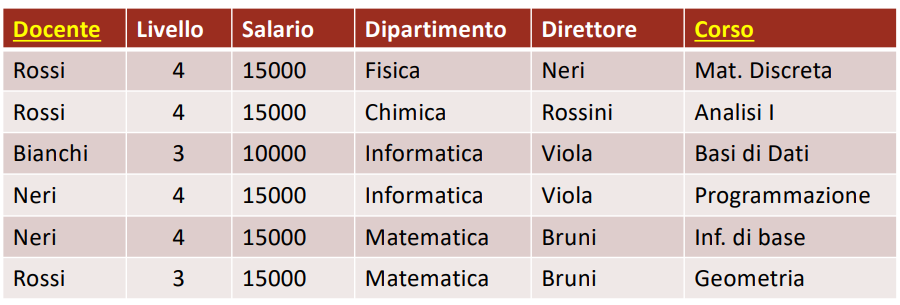
\includegraphics[width=0.7\textwidth]{foto1.png}
\end{center}
Lo stipendio di ciascun docente è ripetuto in tutte le tuple relative, portando ad una \textbf{ridondanza sui dati}. Stesso discorso per il direttore di un dipartimento.\\
Questo problema porta a diverse \textbf{anomalie}, di \textbf{aggiornamento} e di \textbf{cancellazione}. Se dovesse variare lo stipendio, bisogna modificare tutte le tuple del docente. Se invece un docente non ha corsi, bisogna eliminare tutti i suoi dati.\vspace{14pt}\\
Queste problematiche sono causate dall'utilizzo di un'\textbf{unica tabella per rappresentare informazioni eterogenee}.\\
L'errore potrebbe derivare da una \textbf{traduzione non corretta nel modello logico relazionale}, oppure da \textbf{errori durante la progettazione concettuale}.\vspace{14pt}\\
Per risolvere le anomalie viste fin qui si introduce un nuovo concetto del modello relazionale, la \textbf{Dipendenza Funzionale (DF)}:\vspace{14pt}\\
\textit{Definizione}\\
Data una tabella su uno schema \textit{R(X)} e due attributi \textit{Y} e \textit{Z} di \textit{X}. Esiste la \textit{dipendenza funzionale Y --> Z} se per ogni coppia di tuple \textit{t1} e \textit{t2} di \textit{r} con \textit{t1[Y] = t2[Y]}, si ha anche che \textit{t1[Z] = t2[Z]}.\vspace{14pt}\\
\textit{Definizione}\\
Data una tabella su uno schema \textit{R(X)} e due liste di attributi \textit{Y = \{$Y_0$, $Y_1$,\dots, $Y_n$\}} e \textit{Z = \{$Z_0$, $Z_1$,\dots, $Z_n$\}}. Esiste la \textit{dipendenza funzionale Y --> Z} se per ogni coppia di tuple \textit{t1} e \textit{t2} di \textit{r} con \textit{t1[Y] = t2[Y]}, si ha anche che \textit{t1[Z] = t2[Z]}.\vspace{14pt}\\
Si osservi un esempio:
\begin{center}
    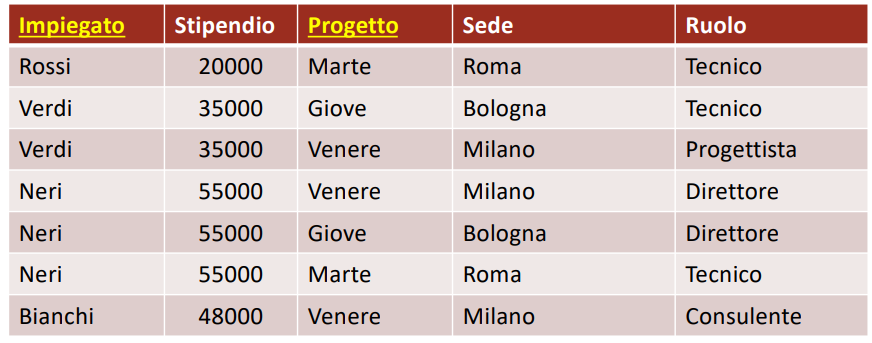
\includegraphics[width=0.7\textwidth]{foto2.png}
\end{center}
Le diverse dipendenze funzionali sono:
\begin{itemize}[label={-}, leftmargin=1cm]
    \itemsep0em
    \item \textbf{\textit{Impiegato --> Stipendio}}: ogni impiegato ha un unico stipendio
    \item \textbf{\textit{Progetto --> Sede}}: ogni progetto ha un'unica Sede
    \item \textbf{\textit{Impiegato --> Impiegato}}: per definizione stessa di dipendenza funzionale
    \item \textbf{\textit{Impiegato Progetto --> Ruolo}}: un impiegato può coprire un solo ruolo per progetto
\end{itemize}
\textbf{Nota Bene}: le dipendenze funzionali sono definite a \textbf{livello di schema} e non a livello di istanza. Inoltre, hanno sempre un \textbf{verso}.\vspace{14pt}\\
Le dipendenze funzionali sono una \textbf{generalizzazione del vincolo di chiave (e di superchiave)}.\vspace{14pt}\\
\textit{Definizione}\\
Data una tabella con schema \textit{R(X)}, con superchiave \textbf{K}. Esiste un vincolo di dipendenza funzionale tra \textit{K} e qualsiasi attributo della tabella o combinazione degli stessi
\begin{center}
    \textit{K --> $X_1$,\quad $X_1$ $\subseteq$ $X$}\\
\end{center}
Si osservi un esempio:
\begin{center}
    
\includegraphics[width=0.7\textwidth]{foto 3.png}
\end{center}
\textit{Impiegato, Progetto} è una \textbf{(super)chiave della relazione}, non possono quindi esistere due tuple con lo stesso valore della coppia <Impiegato, Progetto>.\\
Le dipendenze funzionali sono:
\begin{itemize}[label={-}, leftmargin=1cm]
    \itemsep0em
    \item \textbf{\textit{Impiegato Progetto --> Stipendio}}
    \item \textbf{\textit{Impiegato Progetto --> Sede}}
    \item \textbf{\textit{Impiegato Progetto --> Ruolo}}
    \item \textbf{\textit{Impiegato Progetto --> Sede Ruolo}}
    \item \dots
    \item \textbf{\textit{Impiegato Progetto --> Impiegato Stipendio Progetto Sede Ruolo}}
\end{itemize}
\begin{center}
    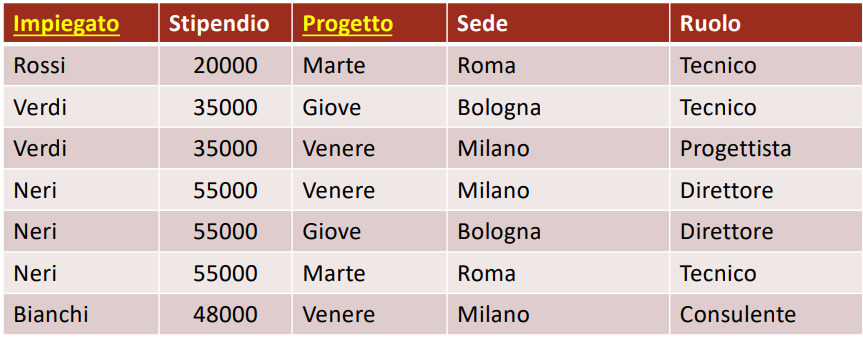
\includegraphics[width=0.7\textwidth]{foto 4.png}
\end{center}
In questo caso le dipendenze funzionali sono:
\begin{itemize}[label={-}, leftmargin=1cm]
    \itemsep0em
    \item \textbf{DF1: \textit{Impiegato --> Stipendio}}
    \item \textbf{DF2: \textit{Progetto --> Sede}}
    \item \textbf{DF3: \textit{Impiegato Progetto --> Ruolo}}
\end{itemize}
Le dipendenze funzionali \textbf{DF1} e \textbf{DF2} sono \textit{cattive}, portando ridondanza sui dati, possibili anomalie(aggiornamento, cancellazione, ecc) nelle operazioni sui dati.\\
La dipendenza funzionale \textbf{DF3} invece è una dipendenza \textit{buona}, non determina ridondanza sui dati.\vspace{14pt}\\
Il motivo per il quale le prime due dipendenze funzionali sono \textit{cattive} è la non presenza di una (super)chiave. Come si può notare, \textbf{DF3} ha sulla sinistra una \textbf{(super)chiave}.\vspace{14pt}\\
\textit{Definizione Forma Normale di BOYCE-CODD (FNBC)}\\
Uno schema \textit{R(X)} si dice in \textbf{forma normale di Boyce e Codd} se per ogni dipendenza funzionale (non ovvia) \textit{Y --> Z} definita su di esso, \textit{Y} è una \textbf{superchiave} di \textit{R(X)}.\vspace{14pt}\\
Se una tabella è in \textbf{FNBC}, non presenta le anomalie e le ridondanze viste fin qui. Al contrario, se una tabella \textbf{non} è in \textit{FNBC}, bisogna trasformarla (\textbf{normalizzarla}), se possibile, in \textit{FNBC}. Due esempi possono essere:
\begin{center}
    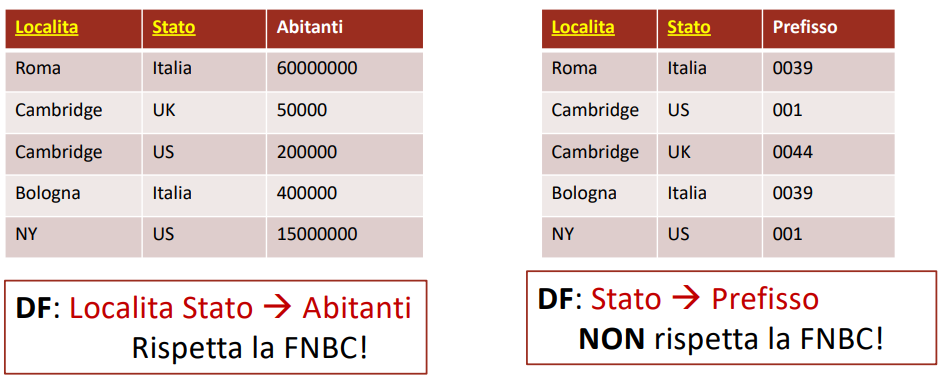
\includegraphics[width=0.7\textwidth]{foto5.png}
\end{center}
Per \textbf{normalizzare} una tabella, si creano \textbf{tabelle separate} per ogni dipendenza funzionale, come è possibile osservare nel seguente esempio:
\begin{center}
    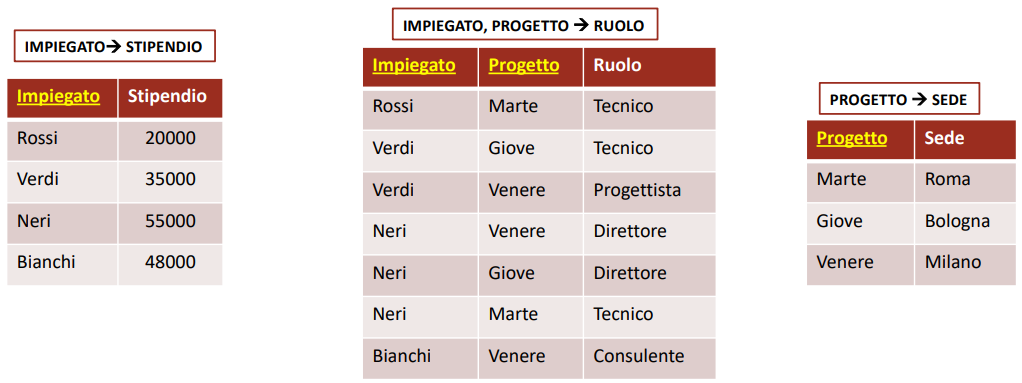
\includegraphics[width=0.7\textwidth]{foto6.png}
\end{center}
Seguendo questa logica, ci si deve chiedere se tutte le decomposizioni sono giuste, o se ci possono essere dei problemi. Si osservino degli esempi:
\begin{center}
    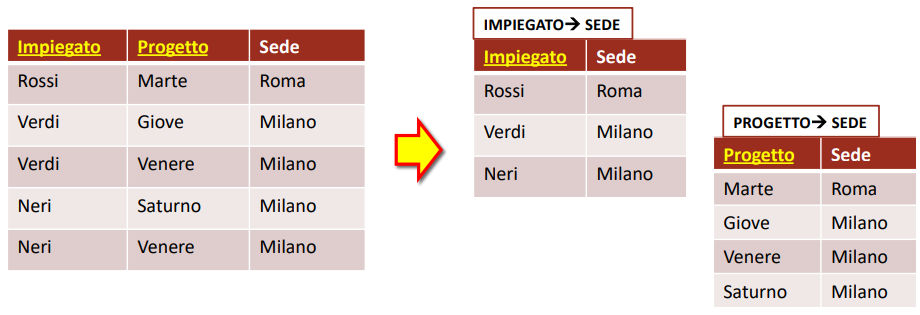
\includegraphics[width=0.7\textwidth]{foto7.png}
\end{center}
In questo caso, \textbf{DF1} implica che ogni impiegato lavora in una sola sede. \textbf{DF2} invece indica che ogni progetto ha la stessa sede.
\begin{center}
    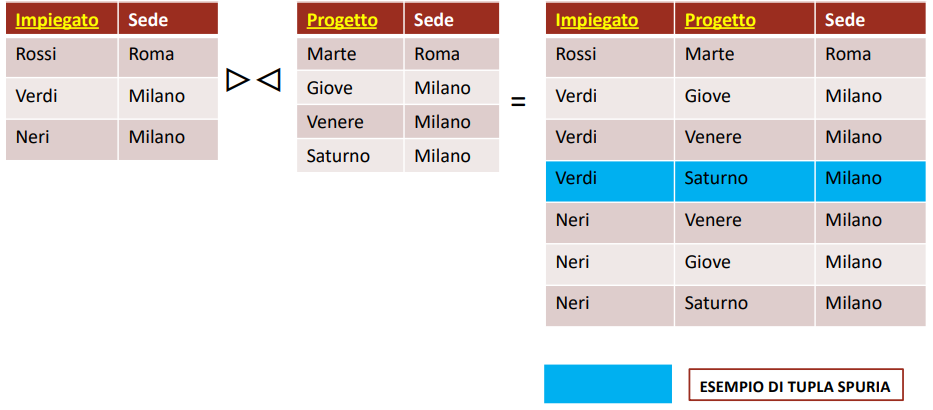
\includegraphics[width=0.7\textwidth]{foto8.png}
\end{center}
Se vengono combinate le due tabelle della decomposizione tramite operatore di join, non si ottiene la tabella di partenza! Si ha quindi una \textbf{decomposizione con perdita/aggiunta}.\vspace{14pt}\\
\textit{Definizione Decomposizione senza perdita}\\
Uno schema \textit{R(X)} si \textbf{decompone senza perdita} negli schemi \textit{R1(X1)} ed \textit{R2(X2)} se, per ogni possibile istanza \textit{r} di \textit{R(X)}, il join naturale delle \textit{X1} ed \textit{X2} produce la tabella di partenza
\begin{center}
    \textit{$\pi X1$(r) $\triangleright$ $\triangleleft$ $\pi X2$(r) = r}\\
\end{center}
In caso di \textbf{decomposizione con perdite/aggiunte}, possono generarsi delle \textbf{tuple spurie dopo il join}.\vspace{14pt}\\
Anche se una decomposizione è senza aggiunte, può comunque presentare dei problemi di \textbf{conservazione delle dipendenze}.\vspace{14pt}\\
Ci si pone quindi la seguente domanda: \textbf{tutte le decomposizioni vanno bene?}\\
La risposta è \textbf{No}. La decomposizione deve soddisfare \textbf{tre proprietà}:
\begin{itemize}[label={-}, leftmargin=1cm]
    \itemsep0em
    \item \textbf{Soddisfacimento della FNBC}: ogni tabella \textbf{deve essere in FNBC}
    \item \textbf{Decomposizione senza perdita}: il join delle tabelle decomposte \textbf{deve produrre la relazione originaria}
    \item \textbf{Conservazione delle dipendenze}: il join delle tabelle decomposte \textbf{deve rispettare tutte le DF dello schema originario}
\end{itemize}
Ci si pone quindi una domanda molto importante. Data una relazione non in \textit{FNBC}, \textbf{è sempre possibile} ottenere una \textbf{decomposizione in FNBC}?\\
La risposta è \textbf{No}. Si consideri un controesempio:
\begin{center}
    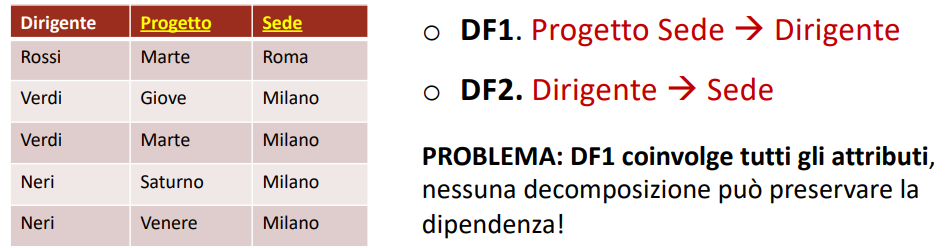
\includegraphics[width=0.7\textwidth]{foto9.png}
\end{center}
Per risolvere casi come questo, si introduce una \textbf{nuova definizione di forma normale} meno restrittiva della forma di \textit{Boyce e Codd}.\vspace{14pt}\\
\textit{Definizione Terza Forma Normale (TFN)}\\
Una tabella \textit{r} è in \textbf{terza forma normale} se per ogni dipendenza funzionale \textit{X --> A} dello schema, \textbf{almeno una delle seguenti condizioni è verificata}:
\begin{itemize}[label={-}, leftmargin=1cm]
    \itemsep0em
    \item \textit{X} è una superchiave di \textit{r}
    \item \textit{A} appartiene ad almeno una chiave \textit{K} di \textit{r}
\end{itemize}
Quindi, la tabella considerata fin qui rispetta la terza forma normale.
\begin{center}
    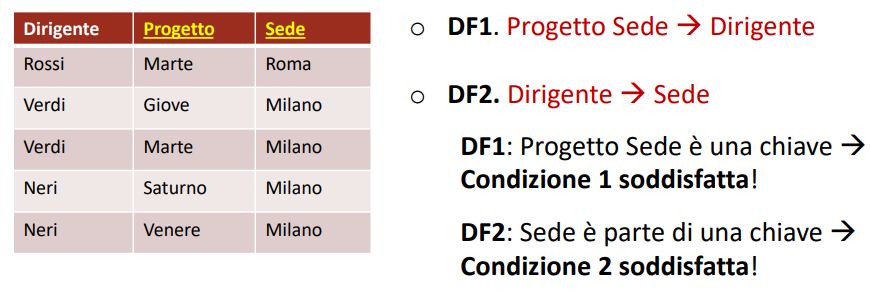
\includegraphics[width=0.7\textwidth]{foto10.png}
\end{center}
Se la tabella è gia in \textit{TFN}, \textbf{non è necessaria alcuna normalizzazione}. Tuttavia, le ridondanze sui dati restano.\vspace{14pt}\\
Confrontando la \textit{TFN} con \textit{FNBC}, si possono notare alcune cose:
\begin{itemize}[label={-}, leftmargin=1cm]
    \itemsep0em
    \item (Svantaggi) La \textit{TFN} è \textbf{meno restrittiva} della \textit{FNBC}, infatti \textbf{tollera alcune ridondanze} ed anomalie sui dati e \textbf{certifica meno la qualità} dello schema ottenuto
    \item (Vantaggi) La \textit{TFN} è \textbf{sempre ottenibile}, qualsiasi sia la tabella. Questo si può raggiungere attraverso l'\textbf{algoritmo di normalizzazione} in \textit{TFN}
\end{itemize}
\subsection*{Algoritmo di normalizzazione in Terza Forma Normale (TFN)}
\large
\textit{Definizione Terza Forma Normale (TFN)}\\
Una tabella \textit{r} è in \textbf{terza forma normale} se per ogni dipendenza funzionale \textit{X --> A} (\underline{non banale}) dello schema, \textbf{almeno una delle seguenti condizioni è verificata}:
\begin{itemize}[label={-}, leftmargin=1cm]
    \itemsep0em
    \item \textit{X} è una superchiave di \textit{r}
    \item \textit{A} appartiene ad almeno una chiave \textit{K} di \textit{r}
\end{itemize}
\textit{Definizione Dipendenza Funzionale Banale}\\
Una dipendenza funzionale \textit{X --> Y} si dice \textbf{banale} se \textit{Y} è contenuto in \textit{X}. Alcuni esempi possono essere:
\begin{itemize}[label={-}, leftmargin=1cm]
    \itemsep0em
    \item \textit{Impiegato Progetto --> Impiegato}
    \item \textit{Impiegato Progetto Sede --> Impiegato Progetto}
\end{itemize}
\textit{Questo genere di dipendenze funzionali non ci interessano, e non le consideriamo come tali nel resto della trattazione!}\vspace{14pt}\\
Data una relazione \textit{r} con schema \textit{R(X)} non in \textit{TFN}, \textbf{normalizzare in TFN} vuol dire decomporre \textit{r} nelle relazioni \textit{$r_1$, $r_2$, $\dots$, $r_n$}, garantendo che:
\begin{itemize}[label={-}, leftmargin=1cm]
    \itemsep0em
    \item Ogni $r_i$ (1 <= i <= n) è in \textit{TFN}
    \item La decomposizione è senza perdite
    \item La decomposizione conserva tutte le dipendenze \textit{F} definite sullo schema \textit{R(X)} di partenza\\
\end{itemize}
L'idea alla base dell'algoritmo di normalizzazione è il seguente:
\begin{itemize}[label={-}, leftmargin=1cm]
    \itemsep0em
    \item \textbf{Semplificare l'insieme di dipendenze F}, rimuovendo quelle non necessarie, e trasformando ogni dipendenza in modo che nella parte destra compaia un singolo attributo
    \item \textbf{Raggruppare gli attributi coinvolti nelle stesse dipendenze}, e costruire le tabelle corrispondenti
    \item \textbf{Assicurarsi che almeno una delle tabella prodotta contenga la chiave} della tabella originaria\\
\end{itemize}
\textit{Definizione Implicazione Funzionale}\\
Dato un insieme di dipendenze funzionali \textit{F}, ed una dipendenza funzionale \textit{f}, diremo che \textbf{F implica f} se ogni tabella che soddisfa \textit{F} soddisfa anche \textit{f}.\vspace{14pt}\\
Si osservi un esempio:\\
\textbf{F}: \{\textit{Impiegato --> Livello}, \textit{Livello --> Stipendio}\}\\
\textbf{f}: \textit{Impiegato --> Stipendio}\\
In questo caso, \textbf{F implica f}!\vspace{14pt}\\
\textit{Definizione Chiusura di una Dipendenza Funzionale}\\
Dato uno schema \textit{R(U)}, con un insieme di dipendenze \textit{F}. Sia \textit{X} un insieme di attributi contenuti in \textit{U}. Si definisce la \textbf{chiusura di X rispetto ad F} (\textbf{$X^+_F$}) come l’insieme degli attributi che dipendono funzionalmente da \textit{X}
\begin{center}
    \textit{$X^+_F$ = \{A | A $\in $ U \quad F implica X --> A\}}
\end{center}
Si osservi un esempio:\\
\textit{R = (ABCDE)}\\
\textit{F = (A --> B, A --> C, C --> D)}\\
Si vuole conoscere la chiusura di A: \textbf{$A^+_F$}\vspace{14pt}\\
\textbf{$A^+_F$ = \{B, C, D\}}\vspace{14pt}\\
Dato quindi in input \textbf{X} (attributi) e \textbf{F} (dipendenze), si ottiene in output \textbf{la chiusura di X rispetto ad F: $X^+_F$}\\
Ad esempio, per verificare se \textit{F implica f : X --> Y}, si può calcolare la chiusura \textit{$X^+_F$}. Se \textbf{Y appartiene ad $X^+_F$}, allora \textbf{F implica f}.\vspace{14pt}\\
Inoltre, data una tabella con schema \textit{R(U)}, l'algoritmo per determinare la chiusura \textit{$X^+_F$} può essere usato anche per \textbf{verificare se X è una superchiave di R}.\\
Infatti, dato uno schema \textit{R(U)}, con un insieme \textit{F} di dipendenze funzionali, allora \textbf{un insieme di attributi K è una (super)chiave di R(U) se F implica K --> U}.\vspace{14pt}\\
Si osservi un esempio:\\
\textit{R = (ABCDE)}\\
\textit{F = (A --> B, BC --> D, B --> E, E --> C)}\\
Se \textit{A} è una chiave allora \textit{F} implica \textit{A -- > ABCDE}\\
\textbf{$A^+_F$ = \{A, B, E, C, D\} quindi A è una chiave!}\vspace{14pt}\\
\textit{Definizione Insiemi di Dipendenze Equivalenti}\\
Dati due insiemi di dipendenze funzionali \textit{$F_1$} ed \textit{$F_2$}, essi si dicono \textbf{equivalenti} se \textit{$F_1$} implica ciascuna dipendenza di \textit{$F_2$} e viceversa.\vspace{14pt}\\
\textit{Definizione Insiemi di Dipendenze Non Ridondanti}\\
Dato un insieme di dipendenze funzionali \textit{F} definito su uno schema \textit{R(U)}, esso si dice \textbf{non ridondante} se non esiste una dipendenza \textit{f} di \textit{F} tale che \textit{F-{f} implica f}.\vspace{14pt}\\
\textit{Definizione Insiemi di Dipendenze Ridotte}\\
Dato un insieme di dipendenze funzionali \textit{F} definito su uno schema \textit{R(U)}, esso si dice \textbf{ridotto} se \textit{(1)} non è ridondante, e \textit{(2)} non è possibile ottenere un insieme \textit{F’} equivalente eliminando attributi dai primi membri di una o più dipendenze di \textit{F}.\vspace{14pt}\\
Dato uno schema \textit{R(U)} con insieme di dipendenze \textit{F}, per trovare una \textbf{copertura ridotta di F} si procede in \textbf{tre passi}:\vspace{14pt}\\
\textit{STEP 1}\\
Sostituire \textit{F} con \textit{$F_1$}, che ha tutti i \textbf{secondi membri composti da un singolo attributo}.\vspace{14pt}\\
\textit{M --> RSDG, MS --> CD, G --> R, D --> S, S --> D, MPD --> AM}\\
\textbf{$F_1$ = \{M --> R, M --> S, M --> D, M --> G, MS --> C, MS --> D, G --> R, \\D --> S, S --> D, MPD --> A, MPD --> M\}}\vspace{14pt}\\
\textit{STEP 2}\\
\textbf{Eliminare gli attributi estranei}.\vspace{14pt}\\
Supponendo di avere \textit{F = \{AB --> C, A --> B\}}, si calcola \textit{$A^+_F$}.\\
\textbf{\textit{$A^+_F$} = ABC}\\
\textbf{C dipende solo da A}, quindi l'attributo \textit{B} in \textit{AB --> C} può essere eliminato preservando l'uguaglianza.\\
\textbf{\textit{$F_1$} = \{A --> C, A --> B\}}\vspace{14pt}\\
In generale, se ho una dipendenza funzionale del tipo: \textbf{AX --> B}, per stabilire se l’attributo \textit{A} può essere eliminato preservando l’uguaglianza \textbf{si calcola \textit{$X^+$} e si verifica se esso include \textit{B}}, nel qual caso \textit{A} può essere eliminato dalla dipendenza.\vspace{14pt}\\
\textit{STEP 3}\\
\textbf{Eliminare le dipendenze non necessarie}.\vspace{14pt}\\
Supponiamo di avere \textit{F = \{B --> C, B --> A, C --> A\}}:\\
\textit{B --> A} è \textbf{ridondante}, in quanto bastano le dipendenze \textit{B --> C} e \textit{C --> A} per capire che \textit{A} dipende da \textit{B}.\\
Formalmente, bisogna dimostrare che \textit{F-\{B --> A\} implica \{B --> A\}, quindi verificare che: $B^+_{F-\{B --> A\}}$ contiene A}\vspace{14pt}\\
In generale, per stabilire se la dipendenza del tipo \textit{X --> A} è ridondante la si elimina da \textit{F}. Successivaente, si calcola $X^+_{F-\{X --> A\}}$, e \textbf{si verifica se tale insieme include ancora A}. Nel caso lo includa, si elimina le dipendenza funzionale \textit{X --> A}.\vspace{14pt}\\
\textit{Algoritmo di normalizzazione in terza forma normale}\\
Dati \textit{R(U)}, ed un insieme di dipendenze \textit{F}, l'\textbf{algoritmo di normalizzazione in terza forma normale} procede come segue:
\begin{enumerate}[leftmargin=1cm]
    \itemsep0em
    \item \textbf{Costruire una copertura ridotta $F_1$ di F}
    \item \textbf{Decomporre $F_1$ nei sottoinsiemi $F_1^{(1)}$, $F_1^{(2)}$, $\dots$, $F_1^{(n)}$}: ad ogni sottoinsieme appartengono dipendenze con gli stessi lati sinistri
    \item \textbf{Se due o più lati sinistri delle dipendenze si implicano a vicenda, si fondono i relativi insiemi}
    \item \textbf{Trasformare ciascun $F_1^{(i)}$ in una tabella $R^{(i)}$} con gli attributi contenuti in ciascuna dipendenza. Il lato sinistro diventa la chiave della relazione
    \item Se nessuna relazione $R^{(i)}$ così ottenuta contiene una chiave \textit{K} di \textit{R(U)}, \textbf{inserire una nuova tabella $R^{(n + 1)}$} contenente gli attributi della chiave\vspace{20pt}\\
\end{enumerate}
Perchè si chiama \textbf{Terza Forma Normale (TFN)}?
\begin{itemize}[label={-}, leftmargin=1cm]
    \itemsep0em
    \item \textbf{Prima Forma Normale (PFN)}: si suppone sia rispettata
    \item \textbf{Seconda Forma Normale (SFN)}: variante debole della \textit{TFN}
\end{itemize}
Procedendo per gradi, si dovrebbe \textbf{normalizzare in PFN, poi in SFN, e quindi in TFN}.\vspace{14pt}\\
\textit{Definizione Seconda Forma Normale}\\
Una relazione \textit{r} con schema \textit{R(U)} è in \textbf{Seconda Forma Normale (SFN)} quando \textbf{non presenta dipendenze parziali}, della forma: \textit{Y --> A}, dove:
\begin{itemize}[label={-}, leftmargin=1cm]
    \itemsep0em
    \item \textit{Y} è un sottoinsieme \textbf{proprio} della chiave
    \item \textit{A} è un qualsiasi sottoinsieme di \textit{R(U)}\\
\end{itemize}
\textit{Definizione Quarta Forma Normale}\\
Una tabella con schema \textit{R(U)} è in \textbf{Quarta Forma Normale (4FN)} se non presenta dipendenze multivalore non banali diverse da una chiave della tabella.\vspace{14pt}\\
\textit{Definizione Quinta Forma Normale}\\
Una tabella con schema \textit{R(U)} è in \textbf{Quinta Forma Normale (5FN)} se non è possible decomporre ulteriormente la tabella senza perdere informazioni.
\end{document}